\section{Whether the estimator matters}
\label{sec:estimator}
Section~\ref{sec:repro} put a magnitude on one specification choice. This
section puts one on the estimation choice it is usually compared against.
Table~\ref{tab:horserace} runs all four covariance estimators through the same
optimiser, on the same review calendar, under the same written constraint set.

\begin{table}[tbp]
\caption{The four covariance estimators under one specification.}
\label{tab:horserace}
\centering\small
\setlength{\tabcolsep}{5pt}
\begin{tabular}{lrrrrrrr}
\toprule
Estimator & Realised vol (\%) & Pred./real. & Bias $b$ & Turnover (\%) & Holdings & Loosened & No trade\\
\midrule
Structural factor model & 15.73 & 0.890 & 1.078 & 12.84 & 109 & 2 & 0\\
Sample & 15.56 & 0.878 & 1.090 & 12.87 & 82 & 6 & 1\\
Ledoit--Wolf & 15.49 & 0.897 & 1.081 & 13.85 & 81 & 5 & 0\\
PCA, Bai--Ng & 15.49 & 0.864 & 1.104 & 14.07 & 84 & 7 & 0\\
\bottomrule
\end{tabular}
\notetext{Each estimator is run through the same constrained optimiser on the same rebalance calendar. They do not face an identical realised constraint set: the last two columns show the relaxation ladder resolving differently across estimators, which is itself an estimator effect. The four realised volatilities span roughly a quarter of a percentage point. Their tracking errors, in Table~\ref{tab:replication}, span 26 basis points as printed there, and that is the figure comparable with the exemption effect in Section~\ref{sec:repro}, both being tracking errors against the same fund. A circular block bootstrap on daily active returns, 21-day blocks, puts the spread at [0.15, 0.40] percentage points. Pred./real. is the ratio of mean predicted to realised annualised volatility, and bias $b$ is the standard deviation of realised return divided by the previous period's predicted standard deviation, computed on the minimum-variance portfolio over 748 observations. The two measure calibration differently and are not interchangeable: $b$ carries a well-specified band of [0.948, 1.052], and all four estimators sit above it. Turnover is the mean one-way figure per rebalance. Loosened counts the rebalances of 29 at which the published ladder put a weaker bound in force, and No trade those at which the ladder was exhausted without reaching a feasible book, so the previous weights were carried forward unchanged. The turnover cap is what binds in almost every case; the sector band was never the bound that had to be loosened.}
\end{table}


One qualification before the numbers. It would be convenient to say the rows
differ in $\Sig$ and in nothing else, and that is not quite true. The last two
columns show the relaxation ladder resolving differently across estimators: the
structural model needed a loosened bound at two of twenty-nine reviews, the
principal-component model at seven, and the sample estimator abandoned one
review altogether. The four runs therefore share a specification without
sharing a realised constraint set. That is itself an estimator effect rather
than a confound to be apologised for, since an estimator that produces
infeasible problems more often is worse on a dimension the realised volatility
does not capture, but the comparison is between specifications-plus-outcomes,
not between matrices held in isolation.

The four realised volatilities span roughly a quarter of a percentage point,
from 15.49\% to 15.73\%. The ordering is not the one the estimators'
statistical properties would predict: the sample covariance, singular by
construction at five hundred names and 156 observations, delivers 15.56\%,
inside the range and below the structural model. Tracking error against the
fund, which is the quantity Section~\ref{sec:repro} measures the exemption
effect in and therefore the one that permits a comparison, spans 5.57\% to
5.83\% in Table~\ref{tab:replication}, a range of 26 basis points. The
exemption effect is 2.10 percentage points. The bootstrap intervals quoted in
Section~\ref{sec:repro} do not overlap.

This is what \citet{dom2025beyond} report for constrained portfolios in
general, and we read our result as a confirmation of theirs in a specific
published constraint set rather than as a new finding. One half of their
result, though, our evidence does not support. Alongside the finding that
constraints make further shrinkage largely redundant, they report that
modelling the time-series dynamics of returns remains statistically relevant
for reducing volatility. The only estimator here that models dynamics is the
two-half-life structural model, and it delivers the highest realised volatility
of the four. We do not read this as a contradiction so much as a difference in
what is being varied: their dynamic estimator alters the covariance process
while holding the cross-sectional structure fixed, whereas ours changes both at
once, adding an industry-and-style factor structure that the other three do not
impose. Separating the two would need a dynamic estimator without the factor
structure, which this study does not run.
\citet{jagannathan2003risk} supply the reason, and it is worth stating
precisely because it is easy to mistake for a claim that estimation does not
matter. Binding weight constraints act as a form of shrinkage. A long-only
constraint with a 1.5\% cap, a five per cent sector band and a ten per cent
turnover limit removes most of the positions through which a covariance
estimate expresses an opinion, so two estimates that disagree substantially
about $\Sig$ can agree almost exactly about the portfolio that survives those
bounds. The estimators are not equivalent. The feasible set is small enough
that their differences cannot reach the result.

\subsection{Reconciling a result that points the other way}
\citet{alonso2020devil} report the opposite ordering, finding that
optimiser-based low-volatility construction is highly sensitive to risk-model
inputs and that small changes in those inputs produce large differences in
sector and stock positioning and in risk exposures. Taken at face value that
contradicts Table~\ref{tab:horserace}, and a reader is entitled to an account
of why.

The two results measure different things, and both can hold. Their sensitivity
is in positioning; ours is in realised volatility. Table~\ref{tab:horserace}
shows positioning differing substantially across estimators: median holdings
run from 81 to 109, mean one-way turnover from 12.84\% to 14.07\%, and the
number of reviews requiring a loosened bound from two to seven. The estimators
do disagree, visibly, about which names to hold and how often to trade them.
What the constraint set does is absorb that disagreement before it reaches
realised risk. On the reading we prefer, their result and ours are the same
phenomenon observed either side of a binding constraint, and the discrepancy is
a reason to report both measures rather than to prefer one.

\subsection{Calibration}
The last column of Table~\ref{tab:horserace} that bears on the model's honesty
is the pair of calibration measures, and they disagree in magnitude while
agreeing in sign.

The ratio of mean predicted to realised volatility runs from 0.864 to 0.897:
every estimator predicts between ten and fourteen per cent less volatility than
its own portfolio went on to deliver. The bias statistic, which standardises
each period's realised return by the previous period's forecast and takes the
standard deviation of the result, runs from 1.078 to 1.104 against a
theoretical band of $[0.948, 1.052]$. Both say the models understate their own
risk; they do not say it by the same amount, because they are computed over
different windows and standardise differently, and the paper is careful to name
which is meant wherever a figure appears.

Figure~\ref{fig:bias} plots the rolling statistic for each estimator.

\begin{figure}[tbp]
\centering
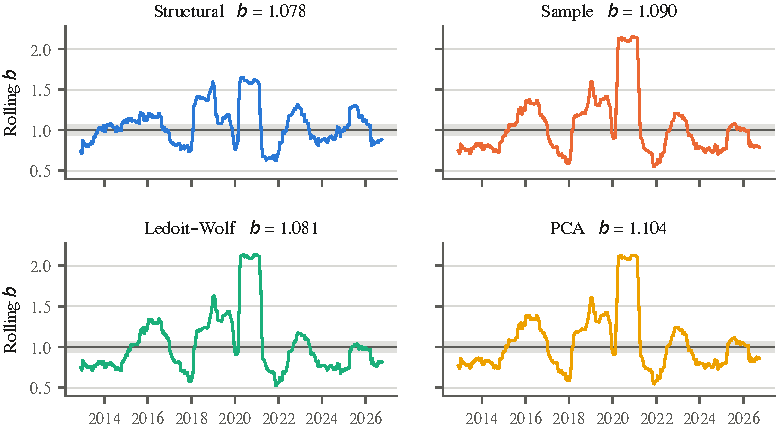
\includegraphics[width=0.94\linewidth]{figures/bias.pdf}
\caption{Rolling bias statistic for the minimum-variance portfolio under each
covariance estimator, on a 52-week window, against the shaded
$1\pm\sqrt{2/T}$ band. The band is a full-sample reference reproduced for
orientation, not a pointwise test for this series: it is derived under
independence, while successive points here share fifty-one weeks of history and
the underlying returns are themselves serially correlated, so excursions are
considerably less surprising than its width suggests. Panel titles give the
full-sample figure. Separate
panels rather than one axis because the three non-structural estimators trace
nearly identical paths and would overplot: the similarity is the point and a
single axis would hide it. All four exceed two during 2020, meaning realised
risk ran at roughly twice the forecast, and all four spend extended periods
below the band as well, so the full-sample figures above one are not a uniform
understatement through time.}
\label{fig:bias}
\end{figure}

Understating risk is not a surprise in a minimum-variance portfolio and it has
a known mechanism. \citet{goldberg2022dispersion} show that excess dispersion
in the leading eigenvector of an estimated covariance matrix propagates through
quadratic optimisation into the risk forecasts of the portfolios it produces,
with the optimiser selecting precisely the directions in which the estimate is
most overconfident. All four of our estimators sit outside the band on the same
side, which is consistent with that account and is not evidence for it over any
other.

There is also a formal counterpart to the argument of this section.
\citet{goldberg2025eigenvector} construct covariance estimates tailored to the
constraints a portfolio will be optimised under, shrinking the leading
eigenvector toward a subspace determined by the constraint gradients. That the
right estimate depends on the constraint set is the same proposition this
section argues empirically from the other direction: when the constraint set is
tight enough, estimates that differ substantially in isolation stop differing
where it counts. Their result is the stronger one, being analytic, and a
replication study is not the place to extend it; we note the connection because
it suggests the finding here is a special case of something general rather than
a feature of this index.

The practical reading is that an optimiser of this kind should not be trusted
to forecast its own risk, whichever of these four matrices sits underneath it.
That conclusion is unchanged across the estimator choice, which is the same
message the realised volatilities deliver from the other direction.
